\chapter{Architecture Description}

% This doesnt have to be a section
\section{Overall description}

%TODO better diagram
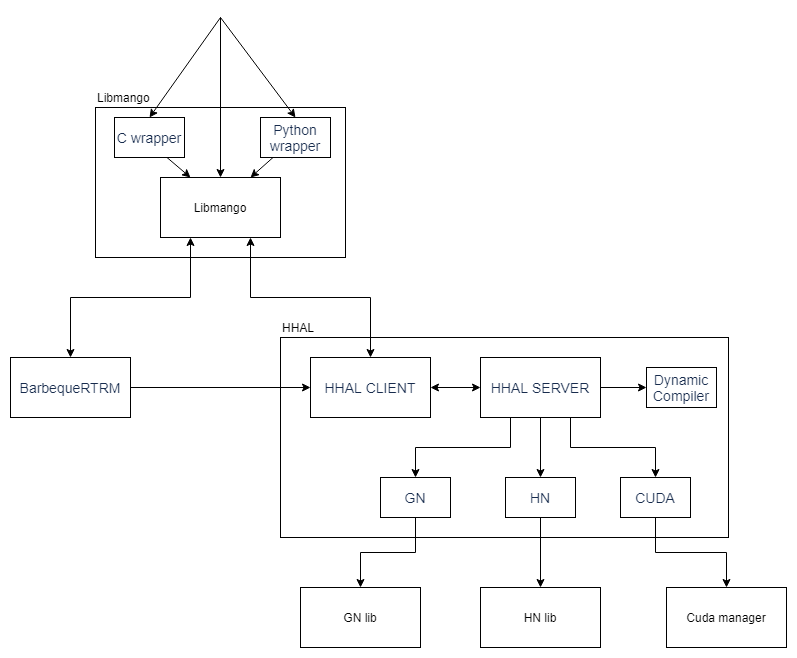
\includegraphics[scale=0.5]{img/architecture.png}

\section{Core elements}
Throughout the multiple MANGO modules, there are a few core elements often present. These are the components necessary to specify and control an user application and its execution. Although their names may vary from module to module, here they are defined as Kernel, Memory Buffer, Event and Task graph.

\subsubsection{Kernel}
In computing, a compute kernel is a routine compiled for high throughput accelerators (such as graphics processing units (GPUs), digital signal processors (DSPs) or field-programmable gate arrays (FPGAs)), separate from but used by a main program (typically running on a central processing unit). \cite{kernel_wikipedia}

The MANGO system manages user defined Kernels and their execution. For a particular Kernel, multiple sources (accelerator specific implementations of the kernel) can be specified. The architectures for which an implementation is available are considered in the kernel-accelerator assignation process by the resource manager. 

As any computer program, a kernel must have the capability of interacting with the outside world in order to perform significant work. This is achieved through the support of kernel arguments.

%TODO styling
Three types of kernel arguments are supported: 
\begin{itemize}
    \item Scalar Argument: A scalar value. For example, an integer.
    \item Buffer Argument: A pointer to a Memory Buffer.
    \item Event Argument: A pointer to an Event data type.
\end{itemize}

\subsubsection{Memory Buffer}
%TODO better diagram
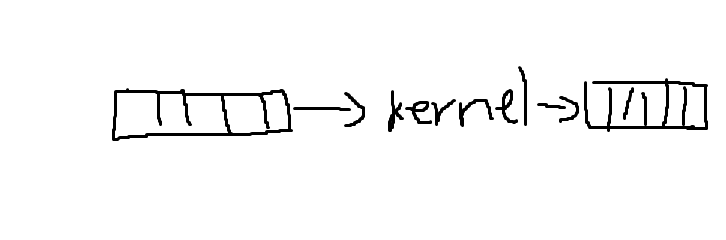
\includegraphics[scale=0.5]{img/kernel_buffer.png}

In computer science, a data buffer (or just buffer) is a region of a physical memory storage used to temporarily store data while it is being moved from one place to another. \cite{buffer_wikipedia}

Kernels read from Input Buffers and write to Output Buffers for inter-kernel and host-kernel data transfering.

A Memory Buffer is defined by the user and allocated by MANGO at the target architectures, where a Kernel that makes use of said Buffer (as either input or output) is assigned.

\subsubsection{Event}

An event is a data structure utilized for communication and synchronization of different parts of the system.

User defined events can be accessed by Kernels through Event Arguments, providing the user with the necessary tools for the implementation of host-kernel or inter-kernel synchronization.

By default, MANGO utilizes kernel termination events for both internal and host synchronization.

\subsubsection{Task Graph}

The Task Graph gives a global picture of the application's behaviour and represents data and control dependencies between Kernels, Memory Buffers and Events. The Task Graph provides the resource manager with the information needed to generate the best feasible resource allocation for the requested QoS. \cite{mango_exploring_manycore_architectures}


\section{Libmango}
\begin{itemize}
    \item 
    api the user interacts with
    \item
    allows software stack developers to easily map high-level programming models on the range of supported accelerators
    \item 
    It achieves this through the usage of Barbecue and HHAL, essentially acting as a layer between user specified models and the rest of the mango system.
    \item
    There are some core elements in the mango system, which are specified by the user and internally handled by libmango:

    explain task graph formed by kernels, buffers, events
    \item 
    The CONTEXT is the main class which holds the state of the host side runtime
    \item
    Subsection: USAGE, how to use libmango (c++)
    \item 
    buffers, events
    \item 
    kernel loading and launching, multiple source support
    \item 
    kernel arguments
\end{itemize}

Libmango is the front-facing module of the MANGO system, hence providing the systems API for user interaction with the underlying components, and acting as an abstraction layer between user defined models and module specific requirements.

The goal of the Libmango module is to allow software stack developers to easily map high-level programming models on the range of supported accelerators. Through the communication with the BarbecueRTRM and HHAL modules, user models are automatically mapped to the supported accelerators in a transparent manner, removing integration complexity from the user's hands.


\section{BarbecueRTRM}

\section{HHAL}

\section{CUDA Manager}

\section{HN}

\section{GN}